\SourcePage{GELFAND-P000453}{73}
\SourceFigure{GELFAND-P000453}{class-arrow}{The arrow by $\Delta^{(0)}$ points down and left toward the first entry.
\par\smallskip\centering\color{black}
\begingroup\color{black}\GelfandFitDiagram{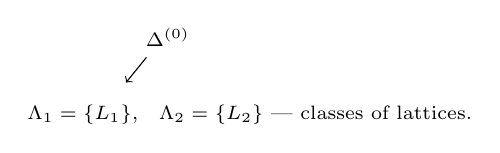
\begin{tikzpicture}[x=1mm,y=1mm,every node/.style={inner sep=0pt,anchor=base west,font=\scriptsize}]
\node (first) at (0,1) {$\Lambda_1=\{L_1\},$};
\node at ([xshift=2.5mm]first.base east) {$\Lambda_2=\{L_2\}$ — classes of lattices.};
\node at (15,10.3) {$\Delta^{(0)}$};
\draw[->] (15.15,8.9) -- (12.55,5.7);
\end{tikzpicture}}\endgroup}
\end{GelfandAdjacentEvidence}
\begin{GelfandAdjacentEvidence}{GELFAND-P000453}{2}


\SourceFigure{GELFAND-P000453}{inclusion-and-residue}{The frame under $L_2\subset L_1$ is open at the top. Two vertical strokes set off the residue field on the right. The left stroke of $F$ is doubled.
\par\smallskip\centering\color{black}
\begingroup\color{black}\GelfandFitDiagram{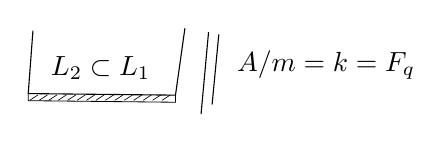
\begin{tikzpicture}[x=1mm,y=1mm]
\node[inner sep=0pt] at (11,7.8) {$L_2\subset L_1$};
\draw (2.4,12.6)--(1.8,4.6)--(20.5,4.4)--(21.7,12.9);
\draw[line width=.3pt] (1.8,4.6)--(1.8,3.7)--(20.5,3.5)--(20.5,4.4);
\foreach \x in {2.0,3.2,...,19.4}{\draw[line width=.24pt] (\x,3.75)--++(1.05,.68);}
\draw (24.7,12.4)--(23.75,2) (26,12.1)--(25.15,3.2);
\node[anchor=west,inner sep=0pt] at (28.25,8.2) {$A/m=k=\mathbb F_q$};
\end{tikzpicture}}\endgroup}
\end{GelfandAdjacentEvidence}
\begin{GelfandAdjacentEvidence}{GELFAND-P000453}{3}


\[
\begin{gathered}
L_1=Ae_1\oplus Ae_2\\
L_2=Ae_1\oplus A\pi^\nu e_2
\end{gathered}
\]
— thus choose the representatives,\quad \uuline{\mbox{$\nu\ge0$}.}
\Unclear{GELFAND-P000453}{representative-word}{The end of the last word is faint. The reading is “представители” (“representatives”).}
\end{GelfandAdjacentEvidence}
\begin{GelfandAdjacentEvidence}{GELFAND-P000453}{4}


$\nu$ is called distance\qquad \uuline{\mbox{$\nu=d(\Lambda_1,\Lambda_2)$}.}

\SourceFigure{GELFAND-P000453}{quotient-cancel}{Three strokes frame the formula below and at the sides. The inscription after the equals sign is heavily cancelled. Its reading is unresolved.
\par\smallskip\centering\color{black}
\begingroup\color{black}\GelfandFitDiagram{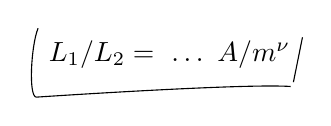
\begin{tikzpicture}[x=1mm,y=1mm]
\node[inner sep=0pt,anchor=base west] (quotient) at (3,5.1)
  {$L_1/L_2={}$ \sout{\ldots}\ $A/m^\nu$};
\path ([yshift=-2.25mm]quotient.south east) coordinate (right);
\draw (1.7,9.3) .. controls (.8,7.1) and (.45,.5) .. (1.5,.55)
  .. controls (9,1.05) and ([xshift=-5mm,yshift=.35mm]right) .. (right);
\draw ([xshift=.35mm,yshift=.55mm]right)--++(1.15,5.7);
\end{tikzpicture}}\endgroup}
\end{GelfandAdjacentEvidence}
\begin{GelfandAdjacentEvidence}{GELFAND-P000453}{5}


\underline{Thm.}\quad This is a corr. def. and is a \underline{distance}.
\begin{center}
\rule[.5ex]{14mm}{.35pt}\enspace$\cdot$\enspace\rule[.5ex]{21mm}{.35pt}
\end{center}

\uuline{Variant:}
\[
L_1/L_2\simeq A/\pi^{\nu_1}A\oplus A/\pi^{\nu_2}A
\]
\Unclear{GELFAND-P000453}{variant-sign}{A single straight stroke lies under the wave. It is set as $\simeq$.}
\end{GelfandAdjacentEvidence}
\begin{GelfandAdjacentEvidence}{GELFAND-P000453}{6}

\[
d(\Lambda_1,\Lambda_2)=|\nu_1-\nu_2|
\]

$\Lambda_1,\Lambda_2$ — neighbors in $\Lambda^0$, if $d(\Lambda',\Lambda^2)=1$.
\Unclear{GELFAND-P000453}{neighbor-notation}{The set has a $\Lambda$ with a small raised circle. In the arguments of $d$, a raised stroke follows the first $\Lambda$ and a raised $2$ follows the second.}
\end{GelfandAdjacentEvidence}
\begin{GelfandAdjacentEvidence}{GELFAND-P000453}{7}


Join them by an edge. We obtain a graph $\Delta$.

\underline{Theorem}:\quad $\Delta$ — a tree (conn. graph without cycles),
and from $\forall$ vertex there issue exactly $q+1$ edges

$\Delta$ is the Lobachevsky pl. — there acts $G$ etc.

\SourceFigure{GELFAND-P000453}{disk-figure}{The outer boundary has a gap at the upper right. The inner arcs and chain follow the visible strokes. A fine mark by the lower left arc resembles an oval. Some joins in the upper right remain uncertain.
\par\smallskip\centering\color{black}
\begingroup\color{black}\GelfandFitDiagram{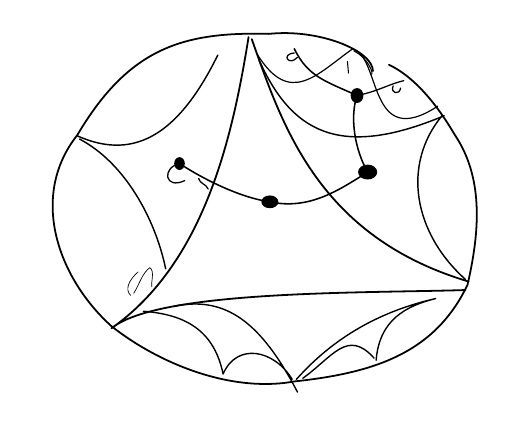
\begin{tikzpicture}[x=.135mm,y=-.135mm,line cap=round,line join=round]
% The outline is broken near the top right, as in the manuscript.
\draw[line width=.64pt] (325,52)
  .. controls (325,33) and (275,12) .. (227,17)
  .. controls (148,15) and (96,29) .. (47,112)
  .. controls (1,170) and (29,247) .. (79,292)
  .. controls (122,326) and (190,355) .. (251,344)
  .. controls (325,336) and (383,318) .. (414,253)
  .. controls (424,209) and (431,155) .. (402,112)
  .. controls (382,78) and (361,56) .. (340,46);
% Main arcs and boundary wedges.
\draw[line width=.65pt] (208,20) .. controls (193,113) and (167,232) .. (79,294)
  .. controls (123,258) and (314,261) .. (412,258);
\draw[line width=.65pt] (211,22) .. controls (240,104) and (274,208) .. (415,250);
\draw[line width=.52pt] (47,113) .. controls (103,138) and (144,108) .. (179,37)
  (49,116) .. controls (91,138) and (120,190) .. (130,238);
\draw[line width=.52pt] (218,42) .. controls (248,108) and (292,136) .. (392,94)
  (390,94) .. controls (352,140) and (363,204) .. (412,248);
\draw[line width=.43pt] (216,36) .. controls (247,86) and (272,55) .. (306,31)
  .. controls (333,39) and (320,128) .. (386,85);
\draw[line width=.37pt] (307,33) .. controls (320,39) and (327,56) .. (323,55)
  (301,43)--(302,54);
\draw[line width=.5pt] (109,278) .. controls (151,281) and (176,298) .. (184,337)
  .. controls (197,307) and (232,314) .. (249,342)
  (139,273) .. controls (186,264) and (219,287) .. (254,354)
  (253,342) .. controls (285,306) and (327,279) .. (384,266)
  .. controls (356,273) and (331,286) .. (328,324)
  (259,341) .. controls (287,321) and (301,294) .. (326,322);
% Inner chain, its short branches, and the separate fine lower-left mark.
\draw[line width=.56pt] (143,139) .. controls (166,154) and (200,171) .. (228,175)
  .. controls (265,183) and (293,164) .. (320,147)
  .. controls (308,126) and (303,96) .. (310,75)
  .. controls (282,62) and (264,58) .. (251,31);
\draw[line width=.46pt] (310,75) .. controls (330,71) and (338,65) .. (354,61)
  (143,139) .. controls (126,143) and (129,164) .. (148,155)
  (161,153) .. controls (162,158) and (168,158) .. (170,163)
  (251,35) .. controls (238,36) and (246,48) .. (254,39)
  (344,66) .. controls (341,73) and (350,75) .. (351,68);
\fill (143,139) ellipse [x radius=5,y radius=6];
\fill (228,175) ellipse [x radius=8,y radius=6];
\fill (320,147) ellipse [x radius=9,y radius=7];
\fill (310,75) ellipse [x radius=6,y radius=7];
\draw[line width=.25pt] (97,263) .. controls (91,257) and (96,248) .. (104,241)
  (100,261) .. controls (105,253) and (108,242) .. (115,237)
  .. controls (120,240) and (116,250) .. (117,255);
\end{tikzpicture}}\endgroup}
\end{GelfandAdjacentEvidence}


\begin{center}
\rule[.5ex]{18mm}{.35pt}\enspace$\bullet$\enspace\rule[.5ex]{21mm}{.35pt}
\end{center}


\Needspace{7\baselineskip}
\begin{GelfandAdjacentEvidence}{GELFAND-P000454}{1}
